\section{Experimental sensitivity}
\label{sec:experiment}

Emphasize discovery potential, not just exclusion sensitivity. May be difficult to combine predictions since some collaborations tend to use exclusion-only predictions e.g. SuperCDMS optimal interval. 

\subsection{Prospects for reaching the neutrino fog}
What are the challenges, R\&D needs for mature technologies to reach the neutrino floor?  Are there any new technologies sensitive to this space that can potentially overcome some of these challenges, and might be competitive with the more mature technologies with sufficient investment?
\subsubsection{Overview of currently-funded sensitivity}


\subsubsection{New technologies}
Scintillating bubble chambers, supercooled detectors, ...
\subsubsection{R\&D to reach the neutrino fog}

\begin{figure}
    \centering
    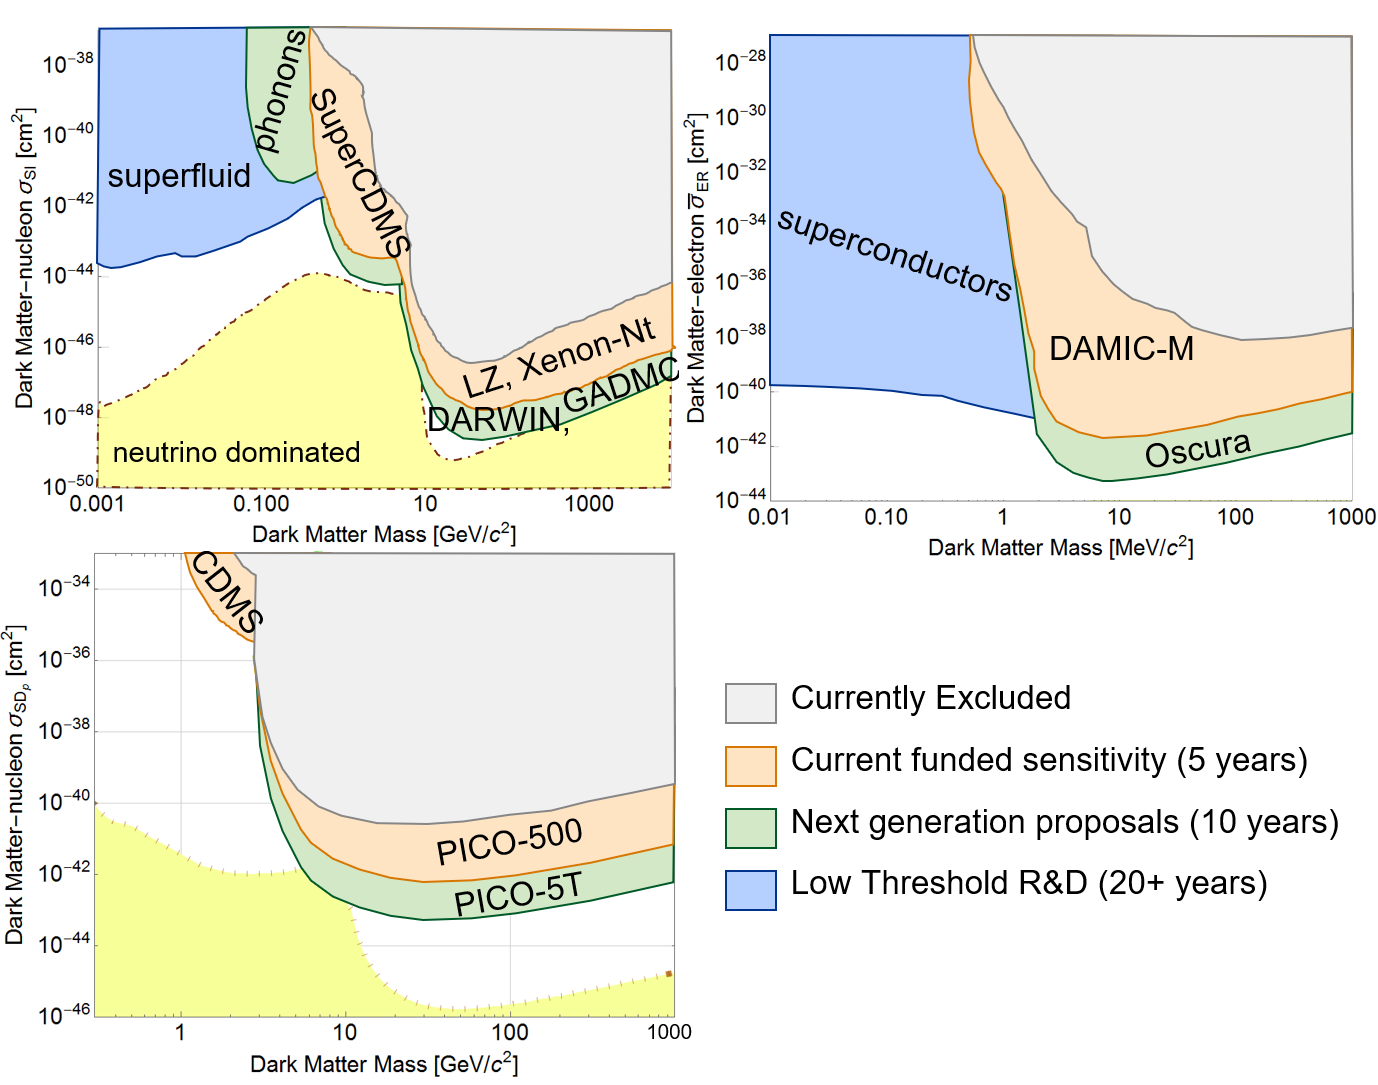
\includegraphics[width=\textwidth]{figures/wimp_sensitivty_cartoon.png}
    \caption{Currently excluded generic spin-independent NR, spin-dependent NR, and ER cross sections. Projected sensitivity of near- amd medium-future experiments. Probably need ER absorption too. Current version is a cartoon and NOT indicative of experiments, labels, timescales, etc.}
    \label{fig:si_sensitivity}
\end{figure}

%Prisca: What would be the umbrella theory here?  Perhaps that belongs in the motivation area of the introduction and we should nest the theory with the type of search (e.g. NR, ER scattering, ER absorption, Dark sector, etc) OR are you imagining that this is basically just a laundry list of what might be searched for?

\subsection{New technologies to push below the neutrino fog}
What is the timescale on which the currently mature technologies might reach the neutrino floor? This sets the timescale by which mature sub-fog technology needs to be developed, which in turn sets the timescale to start heavily prioritizing R\&D. 



\subsubsection{Directional detectors}
Current state of directional detectors. What proposals exist to scale-up mass? 
\begin{figure}
    \centering
    %\includegraphics{}
    \missingfigure{Sensitivity of current and near-future directional detectors}
    \caption{Sensitivity of current and near-future directional detectors}
    \label{fig:directional_sensitivity}
\end{figure}
\subsubsection{Annual modulation?}
\subsubsection{Other technologies?}


\subsection{EFT couplings, dark sector, ...}
For the N most basic EFT couplings, What is the currently-excluded cross section from published results?  \textbf{Is there a mass range that is not being probed in one or more couplings?} Are there new technologies that uniquely address some portion of this parameter space?

\begin{figure}
    \centering
    %\includegraphics{}
    \missingfigure[figheight=16cm]{EFT cross section space excluded}
    \caption{7 or so plots of current and near-future EFT cross-section sensitivity.}
    \label{fig:EFT_sensitivity}
\end{figure}


% Prisca: I suppose our charge is to the neutrino floor. Are ER searches the only thing getting there (under our charge)?   Do we cover only electron scattering (elastic and inelastic) and NOT dark sector stuff and dark photon absorption?   What about getting to the neutrino floor at low mass? This is kind of interesting, because the neutrino floor focus could move the discussion away from pushing to the lowest threshold and open up and interesting examination of what the real limit is to low mass at the largest exposures. Thus, a better organizational principle might be for mass regions instead of NR vs ER.  The theory might be easier to subdivide, too.   But if not, I tried to subdivide ER without low mass. 